% !TEX program = xelatex
% Συμπίεση με: xelatex report.tex
%
% Προαπαιτείται: TeX Live (full ή scheme-medium με polyglossia & fontspec)
% και ελληνική γραμματοσειρά (CMU Serif / Linux Libertine / DejaVu Serif).

\documentclass[11pt,a4paper]{article}

\usepackage{fontspec}
\usepackage{polyglossia}
\setmainlanguage{greek}
\setotherlanguage{english}
\setmainfont{DejaVu Serif}[Scale=0.95]
\setsansfont{DejaVu Sans}[Scale=0.95]
\setmonofont{DejaVu Sans Mono}[Scale=0.85]

\usepackage[a4paper, margin=2.3cm]{geometry}
\usepackage{amsmath, amssymb}
\usepackage{booktabs}
\usepackage{multirow}
\usepackage{array}
\usepackage{caption}
\usepackage{subcaption}
\usepackage{graphicx}
\usepackage{hyperref}
\usepackage{xcolor}
\usepackage{listings}
\usepackage{enumitem}

\hypersetup{
    colorlinks=true,
    linkcolor=blue!60!black,
    urlcolor=blue!60!black,
    citecolor=blue!60!black
}

\lstset{
    basicstyle=\ttfamily\footnotesize,
    breaklines=true,
    frame=single,
    backgroundcolor=\color{gray!8},
    columns=fullflexible,
    keepspaces=true
}

\newcommand{\code}[1]{\texttt{#1}}

\title{\textbf{3η Εργασία στο μάθημα ``Ανάλυση Δεδομένων'' \\ 2025--2026}\\[6pt]
\large Πρόβλεψη του τύπου κρασιού (λευκό / κόκκινο)}
\author{Ονοματεπώνυμο: Ρακοβαλής Παύλος \\
ΑΕΜ: 6931}
\date{\today}

\begin{document}
\maketitle

\section*{Σύνοψη δεδομένων και πειραματικού πλαισίου}

Τα δεδομένα της εργασίας περιέχουν 5\,295 παρατηρήσεις κρασιών με 12
αριθμητικά χημικά χαρακτηριστικά και την κατηγορική μεταβλητή στόχο
\code{wine\_type} (\textit{red} / \textit{white}). Η κατανομή των κλάσεων είναι
έντονα ασύμμετρη:
\begin{itemize}[leftmargin=1.5cm]
    \item \textbf{white}: 3\,991 δείγματα ($\approx 75{,}4\%$),
    \item \textbf{red}:   1\,304 δείγματα ($\approx 24{,}6\%$).
\end{itemize}

Ο διαχωρισμός σε training/test έγινε με αναλογία \textbf{70\%/30\%},
\textbf{stratified} ως προς τη μεταβλητή στόχο, ώστε να διατηρηθεί η αναλογία
των δύο κλάσεων και στα δύο υποσύνολα. Η παράμετρος \code{random\_state}
ορίζεται ίση με τον ΑΕΜ του φοιτητή, δηλαδή \code{random\_state = 6931}.
Έτσι το test set περιέχει $391$ ερυθρά και $1198$ λευκά κρασιά
($n_{\text{test}} = 1589$).

Όλη η ανάλυση υλοποιήθηκε σε \code{Python 3.12} με χρήση των βιβλιοθηκών
\code{pandas}, \code{numpy}, \code{scikit-learn} και \code{matplotlib}.
Σε όλη τη συνέχεια χρησιμοποιείται η σύμβαση \textbf{red = 0} (αρνητική
κλάση) και \textbf{white = 1} (θετική κλάση).

\section{Ερώτημα Α — Πρόβλεψη με μία προβλεπτική μεταβλητή}

Για κάθε μία από τις τρεις προβλεπτικές μεταβλητές
\textbf{Alcohol}, \textbf{pH} και \textbf{Chlorides} εφαρμόστηκαν τρεις
ταξινομητές:
\begin{itemize}[leftmargin=1.5cm]
    \item Logistic Regression (LogReg)
    \item Linear Discriminant Analysis (LDA)
    \item Gaussian Naive Bayes (GNB), με την υπόθεση κανονικής κατανομής για
    το χαρακτηριστικό σε κάθε κλάση.
\end{itemize}

Συνολικά εκπαιδεύτηκαν $3 \times 3 = 9$ μοντέλα.

\subsection{Μέτρα αξιολόγησης που χρησιμοποιήθηκαν}

Λόγω της σημαντικής ανισορροπίας των κλάσεων, η απλή \textit{accuracy}
\emph{δεν} είναι κατάλληλο μέτρο: ένας ταξινομητής που προβλέπει συστηματικά
``white'' πετυχαίνει ήδη accuracy $\approx 0{,}754$. Για τον λόγο αυτό
αναφέρονται επιπλέον:

\begin{itemize}[leftmargin=1.5cm]
    \item \textbf{Balanced Accuracy} =
    $\frac{\text{Sensitivity} + \text{Specificity}}{2}$,
    ανθεκτικό σε ασύμμετρες κλάσεις.
    \item \textbf{Sensitivity (Recall white)} =
    $\dfrac{TP}{TP + FN}$.
    \item \textbf{Specificity (Recall red)} =
    $\dfrac{TN}{TN + FP}$.
    \item \textbf{Precision} ανά κλάση και \textbf{F1} ανά κλάση.
    \item \textbf{AUC (ROC)}: ολοκλήρωμα της καμπύλης ROC, ανεξάρτητο από
    το κατώφλι απόφασης.
\end{itemize}

\subsection{Α(i) Confusion matrices και μέτρα ακρίβειας}

\subsubsection*{(α) Προβλεπτική μεταβλητή: \textit{Alcohol}}

\begin{table}[h!]
\centering
\caption{Confusion matrices στο test set — μεταβλητή \textit{alcohol}.}
\begin{tabular}{lcc|cc|cc}
\toprule
& \multicolumn{2}{c|}{\textbf{LogReg}} &
  \multicolumn{2}{c|}{\textbf{LDA}} &
  \multicolumn{2}{c}{\textbf{GNB}} \\
& pred red & pred white & pred red & pred white & pred red & pred white \\
\midrule
true red    & 0   & 391  & 0   & 391  & 0   & 391 \\
true white  & 0   & 1198 & 0   & 1198 & 0   & 1198 \\
\bottomrule
\end{tabular}
\end{table}

\begin{table}[h!]
\centering
\caption{Μέτρα ακρίβειας — μεταβλητή \textit{alcohol}.}
\begin{tabular}{lccccccc}
\toprule
Method & Acc & BalAcc & AUC & Sens(w) & Spec(r) & F1(w) & F1(r) \\
\midrule
LogReg & 0,7539 & 0,5000 & 0,5219 & 1,0000 & 0,0000 & 0,8597 & 0,0000 \\
LDA    & 0,7539 & 0,5000 & 0,5219 & 1,0000 & 0,0000 & 0,8597 & 0,0000 \\
GNB    & 0,7539 & 0,5000 & 0,5678 & 1,0000 & 0,0000 & 0,8597 & 0,0000 \\
\bottomrule
\end{tabular}
\end{table}

\noindent
\textbf{Σχόλιο:} Και οι τρεις μέθοδοι υπολογίζουν \emph{όριο απόφασης} έξω
από την περιοχή των δεδομένων και προβλέπουν συστηματικά την πλειοψηφική
κλάση (\textit{white}). Η accuracy ($0{,}754$) ταυτίζεται ακριβώς με τη
συχνότητα της πλειοψηφικής κλάσης. Η balanced accuracy ισούται με $0{,}5$,
δηλώνοντας ότι το μοντέλο δεν έχει \emph{καμία} διακριτική ικανότητα.
Το AUC είναι σχεδόν στο τυχαίο όριο ($\approx 0{,}52$ για LogReg/LDA,
$0{,}57$ για GNB), που εξηγείται από
το γεγονός ότι οι μέσες τιμές της \textit{alcohol} στις δύο κλάσεις
είναι σχεδόν ίδιες (10,44 για red έναντι 10,53 για white) σε
σχέση με την τυπική απόκλιση ($\approx 1{,}1$).

\subsubsection*{(β) Προβλεπτική μεταβλητή: \textit{pH}}

\begin{table}[h!]
\centering
\caption{Confusion matrices στο test set — μεταβλητή \textit{pH}.}
\begin{tabular}{lcc|cc|cc}
\toprule
& \multicolumn{2}{c|}{\textbf{LogReg}} &
  \multicolumn{2}{c|}{\textbf{LDA}} &
  \multicolumn{2}{c}{\textbf{GNB}} \\
& pred red & pred white & pred red & pred white & pred red & pred white \\
\midrule
true red    & 36  & 355  & 40  & 351  & 44  & 347 \\
true white  & 30  & 1168 & 42  & 1156 & 47  & 1151 \\
\bottomrule
\end{tabular}
\end{table}

\begin{table}[h!]
\centering
\caption{Μέτρα ακρίβειας — μεταβλητή \textit{pH}.}
\begin{tabular}{lccccccc}
\toprule
Method & Acc & BalAcc & AUC & Sens(w) & Spec(r) & F1(w) & F1(r) \\
\midrule
LogReg & 0,7577 & 0,5335 & 0,6798 & 0,9750 & 0,0921 & 0,8585 & 0,1575 \\
LDA    & 0,7527 & 0,5336 & 0,6798 & 0,9649 & 0,1023 & 0,8547 & 0,1691 \\
GNB    & 0,7520 & 0,5366 & 0,6798 & 0,9608 & 0,1125 & 0,8539 & 0,1826 \\
\bottomrule
\end{tabular}
\end{table}

\noindent
\textbf{Σχόλιο:} Η \textit{pH} φέρνει μέτρια διακριτική ικανότητα
(AUC $\approx 0{,}680$). Το πρόσημο του συντελεστή είναι \emph{αρνητικό}
($\hat{\beta}_1 \approx -4{,}20$ στη LogReg), δηλαδή υψηλότερο pH συσχετίζεται
με κόκκινο κρασί (μέσο pH 3,30 έναντι 3,20). Παρότι η accuracy
αυξάνεται οριακά, η balanced accuracy μένει κοντά στο $0{,}53$, επειδή ο
ταξινομητής εξακολουθεί να μην ``πιάνει'' σχεδόν καθόλου την κλάση red
(specificity $\le 0{,}11$).

\subsubsection*{(γ) Προβλεπτική μεταβλητή: \textit{Chlorides}}

\begin{table}[h!]
\centering
\caption{Confusion matrices στο test set — μεταβλητή \textit{chlorides}.}
\begin{tabular}{lcc|cc|cc}
\toprule
& \multicolumn{2}{c|}{\textbf{LogReg}} &
  \multicolumn{2}{c|}{\textbf{LDA}} &
  \multicolumn{2}{c}{\textbf{GNB}} \\
& pred red & pred white & pred red & pred white & pred red & pred white \\
\midrule
true red    & 26  & 365  & 80  & 311  & 99  & 292 \\
true white  & 23  & 1175 & 38  & 1160 & 38  & 1160 \\
\bottomrule
\end{tabular}
\end{table}

\begin{table}[h!]
\centering
\caption{Μέτρα ακρίβειας — μεταβλητή \textit{chlorides}.}
\begin{tabular}{lccccccc}
\toprule
Method & Acc & BalAcc & AUC & Sens(w) & Spec(r) & F1(w) & F1(r) \\
\midrule
LogReg & 0,7558 & 0,5236 & \textbf{0,9220} & \textbf{0,9808} & 0,0665 & 0,8583 & 0,1182 \\
LDA    & 0,7804 & 0,5864 & \textbf{0,9220} & 0,9683 & 0,2046 & 0,8692 & 0,3143 \\
GNB    & \textbf{0,7923} & \textbf{0,6107} & 0,9214 & 0,9683
       & \textbf{0,2532} & \textbf{0,8755} & \textbf{0,3750} \\
\bottomrule
\end{tabular}
\end{table}

\noindent
\textbf{Σχόλιο:} Η \textit{chlorides} είναι αναμφισβήτητα η ισχυρότερη μονή
μεταβλητή. Η AUC ξεπερνά το $0{,}92$ και για τις τρεις μεθόδους, ενώ
\emph{μόνο εδώ} η balanced accuracy ξεπερνά αξιόλογα το $0{,}5$ — δείκτης
ότι ο ταξινομητής αρχίζει να αναγνωρίζει και την κλάση red. Τα κόκκινα
κρασιά έχουν σχεδόν διπλάσιο μέσο επίπεδο χλωριούχων (0,086 έναντι
0,047), διαφορά που είναι μεγαλύτερη από τις τυπικές αποκλίσεις.

\paragraph{Παρατήρηση για παραμέτρους Gaussian Naive Bayes.}
Για κάθε μία προβλεπτική μεταβλητή, ο GNB εκτιμά μέσο και διασπορά
ξεχωριστά για κάθε κλάση. Στο training set προέκυψαν:

\begin{table}[h!]
\centering
\caption{Παράμετροι Gaussian Naive Bayes ανά κλάση.}
\begin{tabular}{lcccc}
\toprule
Predictor & $\mu_{\text{red}}$ & $\sigma_{\text{red}}$ &
            $\mu_{\text{white}}$ & $\sigma_{\text{white}}$ \\
\midrule
alcohol   & 10,429 & 1,013 & 10,553 & 1,141 \\
pH        & 3,295  & 0,149 & 3,197  & 0,143 \\
chlorides & 0,086  & 0,050 & 0,046  & 0,023 \\
\bottomrule
\end{tabular}
\end{table}

Ιδιαίτερα στη μεταβλητή \textit{chlorides}, η διασπορά της κλάσης red
είναι σχεδόν διπλάσια εκείνης της κλάσης white. Αυτή η διαφορά εκμεταλλεύεται
από τον GNB (που επιτρέπει διαφορετική $\sigma$ ανά κλάση) αλλά \emph{όχι}
από την LDA (που υποθέτει κοινή διασπορά).

\subsection{Α(ii) Καταλληλότερη προβλεπτική μεταβλητή}

Από τα παραπάνω αποτελέσματα προκύπτει σαφέστατα ότι η \textbf{Chlorides}
είναι η καταλληλότερη μονή προβλεπτική μεταβλητή για την πρόβλεψη του τύπου
κρασιού. Η εκτίμηση τεκμηριώνεται στους εξής άξονες:

\begin{enumerate}[leftmargin=1.5cm]
    \item \textbf{AUC.} Η \textit{chlorides} έχει AUC $\approx 0{,}92$, έναντι
    $0{,}68$ της \textit{pH} και $0{,}52\sim 0{,}57$ της \textit{alcohol}.
    Το AUC είναι
    το πιο ``δίκαιο'' μέτρο, καθώς αξιολογεί τη διακριτική ικανότητα του
    ταξινομητή ανεξάρτητα από το επιλεγμένο κατώφλι.

    \item \textbf{Λόγος σήματος προς θόρυβο.} Η απόσταση των μέσων τιμών
    των δύο κλάσεων ως προς τη μέση τυπική απόκλιση είναι:
    \[
    d_{\text{chlorides}} \approx \frac{0{,}086 - 0{,}046}{0{,}037} \approx 1{,}1,
    \quad
    d_{\text{pH}} \approx \frac{0{,}10}{0{,}146} \approx 0{,}68,
    \quad
    d_{\text{alcohol}} \approx \frac{0{,}12}{1{,}08} \approx 0{,}11.
    \]
    Δηλαδή η chlorides προσφέρει \textit{σήμα} τάξης μεγέθους ίσο με τη
    διασπορά, ενώ η alcohol πρακτικά κανένα.

    \item \textbf{Balanced Accuracy.} Με την \textit{chlorides} η balanced
    accuracy φτάνει το $0{,}61$ (GNB), ενώ με τις άλλες δύο μεταβλητές
    παραμένει κοντά στο τυχαίο όριο $0{,}5$.

    \item \textbf{F1 για την κλάση red.} Μόνο η \textit{chlorides}
    επιτρέπει αξιοπρεπή ταξινόμηση της μειοψηφικής κλάσης
    (F1\textsubscript{red} έως $0{,}38$). Με τις άλλες μεταβλητές, η
    F1\textsubscript{red} κυμαίνεται μεταξύ $0$ και $0{,}18$.

    \item \textbf{Φυσική / οινολογική ερμηνεία.} Τα ερυθρά κρασιά
    παράγονται με μάκρωση επί της φλούδας, διαδικασία που τυπικά αυξάνει
    τη συγκέντρωση χλωριούχων αλάτων. Είναι λοιπόν αναμενόμενο και
    ερμηνεύσιμο φυσικά να αποτελεί η \textit{chlorides} τον ισχυρότερο
    διακριτή των δύο τύπων.
\end{enumerate}

\subsection{Α(iii) Σύγκριση μεθόδων με προβλεπτική την Chlorides}

Στην ενότητα αυτή εξετάζουμε αν οι τρεις μέθοδοι ταξινόμησης παρουσιάζουν
σημαντική διαφορά στην επίδοση όταν χρησιμοποιείται \emph{αποκλειστικά}
η μεταβλητή \textit{chlorides}.

\subsubsection*{Διαφορές στις προβλέψεις του test set}

\begin{table}[h!]
\centering
\caption{Επίδοση των τριών μεθόδων στο test set με μοναδική προβλεπτική
την \textit{chlorides}.}
\begin{tabular}{lccccc}
\toprule
Method & Accuracy & BalAcc & AUC & Sens(w) & Spec(r) \\
\midrule
LogReg      & 0,7558 & 0,5236 & \textbf{0,9220} & \textbf{0,9808} & 0,0665 \\
LDA         & 0,7804 & 0,5864 & \textbf{0,9220} & 0,9683 & 0,2046 \\
\textbf{GNB} & \textbf{0,7923} & \textbf{0,6107}
            & 0,9214 & 0,9683 & \textbf{0,2532} \\
\bottomrule
\end{tabular}
\end{table}

\subsubsection*{Έλεγχος στατιστικής σημαντικότητας: McNemar test}

Ο έλεγχος του \textit{McNemar} είναι ζευγαρωτός: συγκρίνει τις σωστές /
λανθασμένες προβλέψεις δύο ταξινομητών στα \emph{ίδια} test δείγματα.
Η μηδενική υπόθεση είναι ότι τα δύο μοντέλα έχουν την ίδια πιθανότητα
λάθους.

\begin{table}[h!]
\centering
\caption{McNemar test (paired) — \textit{chlorides} ως μοναδική
προβλεπτική.}
\begin{tabular}{lccc}
\toprule
Σύγκριση (A vs B) & A σωστό \& B λάθος & A λάθος \& B σωστό & p-value \\
\midrule
LogReg vs LDA   & 15 & 54 & $2{,}6\times 10^{-6}$ \\
LogReg vs GNB   & 15 & 73 & $2{,}6\times 10^{-10}$ \\
LDA    vs GNB   &  0 & 19 & $3{,}8\times 10^{-6}$ \\
\bottomrule
\end{tabular}
\end{table}

Και οι τρεις p-τιμές είναι μικρότερες του $\alpha = 0{,}05$, άρα οι
διαφορές στην επίδοση είναι \textbf{στατιστικά σημαντικές}. Η σχέση
που προκύπτει είναι:
\[
\text{GNB}\;\succ\;\text{LDA}\;\succ\;\text{LogReg}
\]
με την έννοια ότι ο επόμενος πετυχαίνει \emph{περισσότερες} σωστές
προβλέψεις από τον προηγούμενο.

\subsubsection*{Επιβεβαίωση με 10-fold Stratified Cross-Validation}

Για να αποκλειστεί η εξάρτηση από συγκεκριμένο διαχωρισμό, τα μοντέλα
αξιολογήθηκαν επιπλέον με 10-fold stratified cross-validation σε όλο
το dataset:

\begin{table}[h!]
\centering
\caption{10-fold Stratified CV (μέσος $\pm$ τυπική απόκλιση).}
\begin{tabular}{lccc}
\toprule
Method & Accuracy & Balanced Accuracy & AUC \\
\midrule
LogReg      & $0{,}7535 \pm 0{,}0053$ & $0{,}5195 \pm 0{,}0105$
            & $0{,}9184 \pm 0{,}0124$ \\
LDA         & $0{,}7817 \pm 0{,}0098$ & $0{,}5859 \pm 0{,}0180$
            & $0{,}9184 \pm 0{,}0124$ \\
\textbf{GNB} & $\mathbf{0{,}7915 \pm 0{,}0098}$
            & $\mathbf{0{,}6082 \pm 0{,}0181}$
            & $0{,}9176 \pm 0{,}0106$ \\
\bottomrule
\end{tabular}
\end{table}

Τα CV αποτελέσματα επιβεβαιώνουν την κατάταξη: ο GNB έχει τη μεγαλύτερη
μέση accuracy και balanced accuracy, η LDA ακολουθεί πολύ κοντά, ενώ η
LogReg υπολείπεται κατά $\approx 4$ ποσοστιαίες μονάδες.

\subsubsection*{Συζήτηση: γιατί διαφέρουν παρόλο που το AUC είναι σχεδόν ίδιο;}

Όλες οι μέθοδοι παράγουν \emph{ίδιας ποιότητας διάταξη} πιθανοτήτων
(AUC $\approx 0{,}92$ και για τις τρεις). Άρα η ικανότητά τους να
διαχωρίσουν τις δύο κλάσεις σε επίπεδο πιθανοτήτων είναι ισοδύναμη.
Οι διαφορές στην accuracy εντοπίζονται στο \emph{σημείο} όπου τοποθετείται
το όριο απόφασης (κατώφλι $0{,}5$ στην προβλεπόμενη πιθανότητα):

\begin{itemize}[leftmargin=1.5cm]
    \item \textbf{LogReg.} Μοντελοποιεί άμεσα το $\log\!\frac{p}{1-p}$ ως
    γραμμική συνάρτηση της chlorides. Λόγω της ασυμμετρίας των κλάσεων
    και του γεγονότος ότι η μεγάλη πυκνότητα των white τιμών συγκεντρώνεται
    σε μικρά chlorides, το όριο $p=0{,}5$ μετατοπίζεται σε υψηλή τιμή
    chlorides — με αποτέλεσμα σχεδόν όλα τα δείγματα να ταξινομούνται
    ως white.
    \item \textbf{LDA.} Υποθέτει κανονική κατανομή ανά κλάση με
    \emph{κοινή} διασπορά. Ενσωματώνει ρητά τα priors (3:1 υπέρ της
    white) στον υπολογισμό των posterior, αλλά συγχρόνως ισορροπεί
    το όριο σε σημείο που λαμβάνει υπόψη τις μέσες τιμές των δύο κλάσεων.
    \item \textbf{GNB.} Επιτρέπει \emph{διαφορετική} διασπορά ανά κλάση.
    Αξιοποιεί το γεγονός ότι $\sigma_{\text{red}} \approx 2 \cdot
    \sigma_{\text{white}}$, ώστε η posterior $P(\text{red}\mid x)$
    να αυξάνει πιο γρήγορα όταν η τιμή χλωριούχων ξεπερνά τη μέση τιμή
    των white. Έτσι τοποθετεί το όριο σε χαμηλότερο σημείο και ``πιάνει''
    περισσότερα κόκκινα δείγματα.
\end{itemize}

\subsubsection*{Συμπέρασμα του Α(iii)}

\begin{itemize}[leftmargin=1.5cm]
    \item Υπάρχει \textbf{σημαντική (στατιστικά) διαφορά} στην επίδοση
    των μεθόδων όταν χρησιμοποιείται μόνο η \textit{chlorides}.
    \item Καλύτερη απόδοση παρουσιάζει ο \textbf{Gaussian Naive Bayes}
    (accuracy $\approx 0{,}79$, balanced accuracy $\approx 0{,}61$,
    F1\textsubscript{red} $\approx 0{,}38$).
    \item Η διαφορά οφείλεται στην ικανότητά του GNB να μοντελοποιεί
    διαφορετικές διασπορές ανά κλάση, σε αντίθεση με τη LDA που υποθέτει
    κοινή διασπορά.
    \item Η LogReg, παρότι έχει \emph{ίδιο} AUC με τις άλλες, λειτουργεί
    πρακτικά ως majority-class predictor στο κατώφλι $0{,}5$ και είναι
    η χειρότερη επιλογή στη συγκεκριμένη ρύθμιση.
\end{itemize}

\section{Ερώτημα Β — Πρόβλεψη με όλες τις προβλεπτικές μεταβλητές}

Στο Ερώτημα Β χρησιμοποιούμε ως προβλεπτικές μεταβλητές \emph{όλες} τις
χημικές μετρήσεις του dataset, εξαιρώντας μόνο τις δύο μη-προβλεπτικές
στήλες: τη μεταβλητή στόχο \code{wine\_type} και τη μεταβλητή \code{quality}
(όπως ορίζει η εκφώνηση). Καταλήγουμε έτσι σε $p = 11$ προβλεπτικές:
\textit{fixed acidity, volatile acidity, citric acid, residual sugar,
chlorides, free sulfur dioxide, total sulfur dioxide, density, pH,
sulphates, alcohol}.

Διατηρούμε τον ίδιο διαχωρισμό 70\%/30\% stratified με
\code{random\_state=6931}, συνεπώς το test set περιέχει
$391$ red και $1198$ white δείγματα ($n_{\text{test}} = 1589$).

\subsection{Μέθοδοι και προεπεξεργασία}

Εκπαιδεύτηκαν πέντε ταξινομητές:
\begin{enumerate}[leftmargin=1.5cm]
    \item \textbf{KNN}, με την παράμετρο $K$ να επιλέγεται μέσω
    \emph{5-fold Stratified CV} στο training set.
    \item \textbf{Logistic Regression} (\code{lbfgs}, \code{max\_iter=5000}).
    \item \textbf{Linear Discriminant Analysis (LDA)}.
    \item \textbf{Quadratic Discriminant Analysis (QDA)}, με ελαφρά
    κανονικοποίηση \code{reg\_param} = $10^{-3}$ για την αντιμετώπιση
    οριακά μη-αντιστρέψιμου πίνακα συνδιακύμανσης.
    \item \textbf{Gaussian Naive Bayes (GNB)}.
\end{enumerate}

\paragraph{Σχετικά με την κανονικοποίηση δεδομένων.}
Οι προβλεπτικές μεταβλητές διαφέρουν δραστικά σε κλίμακα
(π.χ. \textit{total sulfur dioxide} εύρους έως $\sim 440$ έναντι
\textit{chlorides} εύρους $\sim 0{,}6$). Συνεπώς:
\begin{itemize}[leftmargin=1.5cm]
    \item \textbf{KNN}: \emph{απαραίτητη} τυποποίηση
    (\code{StandardScaler}), διότι ο αλγόριθμος βασίζεται σε ευκλείδειες
    αποστάσεις και θα κυριαρχούσαν οι μεταβλητές με μεγάλη κλίμακα.
    \item \textbf{Logistic Regression}: \emph{συνιστάται} τυποποίηση για
    αριθμητική σταθερότητα και ταχύτερη σύγκλιση του \code{lbfgs}.
    \item \textbf{LDA, QDA, GNB}: είναι αμετάβλητοι σε γραμμική
    αλλαγή κλίμακας ανά μεταβλητή, οπότε η τυποποίηση δεν είναι
    απαραίτητη (αλλά και δεν επηρεάζει αρνητικά).
\end{itemize}
Στην υλοποίηση, η τυποποίηση ενσωματώθηκε σε \code{Pipeline} ώστε ο
\code{StandardScaler} να εκτιμάται μόνο στο training fold του CV,
αποφεύγοντας \textit{data leakage}.

\subsection{Επιλογή της παραμέτρου $K$ για τον KNN}

Με 5-fold stratified cross-validation στο training set (3\,706 δείγματα)
και $K \in \{1, 2, \ldots, 30\}$, η μέση CV accuracy μεγιστοποιείται
στο $\boxed{K = 9}$ με τιμή $0{,}9692$ (Σχήμα~\ref{fig:knncv}).

\begin{figure}[h!]
\centering
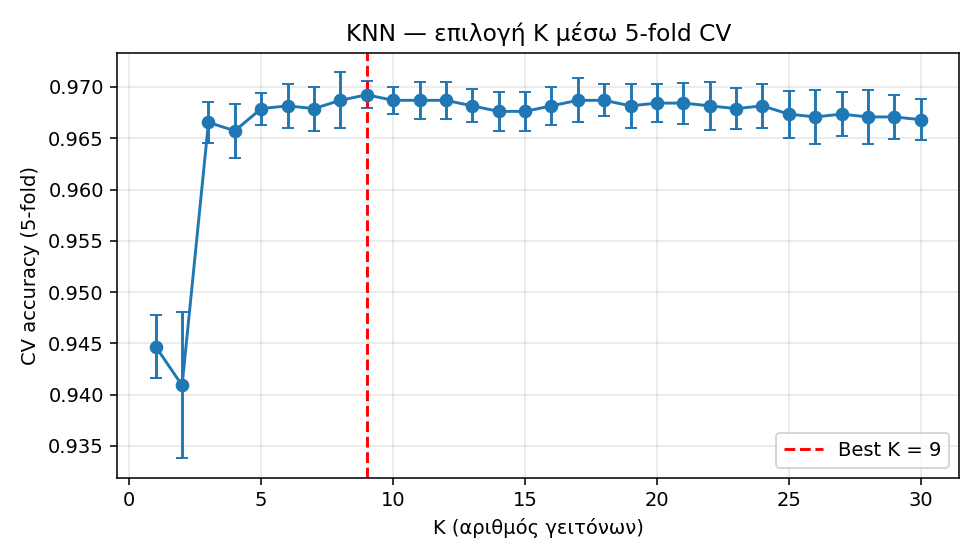
\includegraphics[width=0.85\textwidth]{Q2_knn_cv.png}
\caption{Επιλογή της βέλτιστης τιμής $K$ για τον KNN μέσω 5-fold
stratified CV. Το κόκκινο διακεκομμένο δείχνει τη βέλτιστη τιμή
$K = 9$. Οι μπάρες σφάλματος αντιστοιχούν στην τυπική απόκλιση
μεταξύ των 5 folds.}
\label{fig:knncv}
\end{figure}

\noindent
\textbf{Σχόλιο:} Η καμπύλη CV accuracy εμφανίζει χαρακτηριστική
συμπεριφορά: οι πολύ μικρές τιμές $K \in \{1,2\}$ υποαποδίδουν
($\sim 0{,}94$) λόγω υψηλής διασποράς (overfitting), σταθεροποιείται
από $K \approx 5$ και άνω σε ένα ``plateau'' γύρω στο $0{,}967$, με
τη μέγιστη τιμή στο $K = 9$. Επειδή οι διαφορές μετά το $K \approx 5$
είναι μικρότερες από την τυπική απόκλιση, η επιλογή $K = 9$ είναι
ουσιαστικά ισοδύναμη με κάθε τιμή στο διάστημα $[5, 20]$.

\subsection{Β(i) Confusion matrices στο test set}

Για κάθε μέθοδο παρουσιάζεται ο πίνακας σύγχυσης στα 1\,589 δείγματα
του test set (red = αρνητική, white = θετική κλάση).

\begin{table}[h!]
\centering
\caption{Confusion matrices στο test set — όλες οι μέθοδοι του Ερωτήματος Β.}
\begin{tabular}{lcc|cc|cc|cc|cc}
\toprule
& \multicolumn{2}{c|}{\textbf{KNN ($K=9$)}}
& \multicolumn{2}{c|}{\textbf{LogReg}}
& \multicolumn{2}{c|}{\textbf{LDA}}
& \multicolumn{2}{c|}{\textbf{QDA}}
& \multicolumn{2}{c}{\textbf{GNB}} \\
& pred r & pred w & pred r & pred w & pred r & pred w
& pred r & pred w & pred r & pred w \\
\midrule
true red    & 369 &   22 & 363 &   28 & 363 &   28 & 357 &   34 & 358 &   33 \\
true white  &  25 & 1173 &  27 & 1171 &  23 & 1175 &  36 & 1162 &  56 & 1142 \\
\bottomrule
\end{tabular}
\end{table}

\subsection{Β(ii) Μέτρα ακρίβειας}

Παρουσιάζονται για κάθε μέθοδο τα ίδια μέτρα με το Ερώτημα Α
(accuracy, balanced accuracy, sensitivity, specificity, F1 ανά κλάση,
AUC), διατηρώντας τη διάκριση red/white λόγω της σημαντικής
ανισορροπίας των κλάσεων.

\begin{table}[h!]
\centering
\caption{Μέτρα ακρίβειας στο test set — όλες οι 11 προβλεπτικές μεταβλητές.}
\begin{tabular}{lccccccc}
\toprule
Method & Acc & BalAcc & AUC & Sens(w) & Spec(r) & F1(w) & F1(r) \\
\midrule
\textbf{KNN ($K{=}9$)}  & \textbf{0,9704} & \textbf{0,9614}
                        & 0,9664 & 0,9791 & \textbf{0,9437}
                        & \textbf{0,9804} & \textbf{0,9401} \\
LogReg                  & 0,9654 & 0,9529 & \textbf{0,9692}
                        & 0,9775 & 0,9284 & 0,9771 & 0,9296 \\
LDA                     & 0,9679 & 0,9546 & 0,9678
                        & \textbf{0,9808} & 0,9284 & 0,9788 & 0,9344 \\
QDA                     & 0,9559 & 0,9415 & 0,9605
                        & 0,9699 & 0,9130 & 0,9708 & 0,9107 \\
GNB                     & 0,9440 & 0,9344 & 0,9575
                        & 0,9533 & 0,9156 & 0,9625 & 0,8894 \\
\bottomrule
\end{tabular}
\end{table}

\noindent
Με όλες τις προβλεπτικές μεταβλητές διαθέσιμες, και οι πέντε μέθοδοι
επιτυγχάνουν \emph{εξαιρετική} επίδοση: η accuracy κυμαίνεται από
$0{,}9440$ (GNB) έως $0{,}9704$ (KNN), η balanced accuracy ξεπερνά
παντού το $0{,}93$ — δραματική βελτίωση σε σχέση με το Ερώτημα Α
($\le 0{,}61$). Η ισχυρή ικανότητα ταξινόμησης οφείλεται στο γεγονός
ότι οι 11 χημικές μεταβλητές προσφέρουν \emph{συμπληρωματική}
πληροφορία (π.χ. \textit{volatile acidity}, \textit{total sulfur
dioxide}, \textit{residual sugar}), που μαζί διαχωρίζουν σχεδόν
τέλεια τα ερυθρά από τα λευκά κρασιά.

\subsection{Β(iii) Καμπύλες ROC και AUC}

\begin{figure}[h!]
\centering
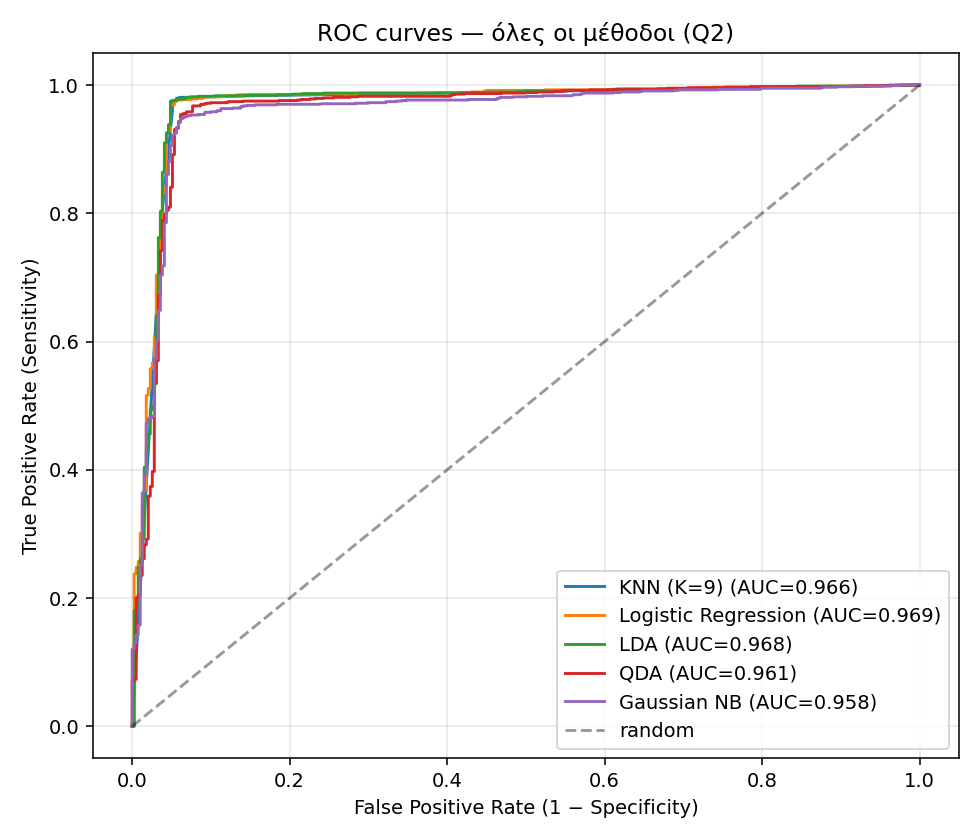
\includegraphics[width=0.78\textwidth]{Q2_roc.png}
\caption{Καμπύλες ROC των πέντε μεθόδων στο test set (Ερώτημα Β).
Η διακεκομμένη μαύρη γραμμή αντιστοιχεί σε τυχαίο ταξινομητή
($AUC = 0{,}5$).}
\label{fig:rocB}
\end{figure}

Οι τιμές AUC συνοψίζονται παρακάτω:

\begin{table}[h!]
\centering
\caption{AUC ανά μέθοδο (Ερώτημα Β).}
\begin{tabular}{lc}
\toprule
Method & AUC \\
\midrule
Logistic Regression & \textbf{0,9692} \\
LDA                 & 0,9678 \\
KNN ($K = 9$)       & 0,9664 \\
QDA                 & 0,9605 \\
Gaussian NB         & 0,9575 \\
\bottomrule
\end{tabular}
\end{table}

\noindent
Όλες οι μέθοδοι έχουν AUC $> 0{,}95$, δηλαδή σχεδόν τέλεια
διακριτική ικανότητα. Παρατηρείται ότι:
\begin{itemize}[leftmargin=1.5cm]
    \item Οι \textbf{γραμμικές} μέθοδοι (LogReg, LDA) και ο
    \textbf{KNN} αποτελούν την ``επάνω'' ομάδα με
    AUC $\in [0{,}966, 0{,}970]$.
    \item Οι QDA και GNB πέφτουν χαμηλότερα ($0{,}96$ και $0{,}958$).
    \item Στο επίπεδο των πιθανοτήτων, η Logistic Regression έχει
    οριακά την υψηλότερη AUC ($0{,}9692$), αλλά \emph{σε επίπεδο
    απόφασης} (κατώφλι $0{,}5$) ο KNN πετυχαίνει την υψηλότερη
    accuracy και balanced accuracy χάρη σε καλύτερη \textit{specificity}
    στην κλάση red.
\end{itemize}

\subsection{Β(iv) Στατιστική σύγκριση των μεθόδων: McNemar test}

Για τον έλεγχο σημαντικής διαφοράς ανάμεσα στις πέντε μεθόδους
εφαρμόστηκε ο ζευγαρωτός έλεγχος του \textit{McNemar} σε όλα τα
$\binom{5}{2} = 10$ ζεύγη. Σε κάθε ζεύγος καταγράφονται:
$b_{AB}$ = δείγματα όπου σωστή \emph{μόνο} η A και $b_{BA}$ =
δείγματα όπου σωστή \emph{μόνο} η B. Λόγω σχετικά μικρών συνολικών
ασυμφωνιών χρησιμοποιήθηκε η ακριβής (\textit{exact}) εκδοχή του
test.

\begin{table}[h!]
\centering
\caption{McNemar test (paired) — Ερώτημα Β. Έντονο = $p < 0{,}05$.}
\begin{tabular}{lccc}
\toprule
Σύγκριση (A vs B) & $b_{AB}$ & $b_{BA}$ & $p$-value \\
\midrule
KNN vs LogReg   & 13 &  5 & 0,096 \\
KNN vs LDA      &  9 &  5 & 0,424 \\
KNN vs QDA      & 27 &  4 & \textbf{$7{,}8 \times 10^{-5}$} \\
KNN vs GNB      & 44 &  2 & \textbf{$1{,}5 \times 10^{-9}$} \\
LogReg vs LDA   &  2 &  6 & 0,289 \\
LogReg vs QDA   & 21 &  6 & \textbf{$7{,}1 \times 10^{-3}$} \\
LogReg vs GNB   & 38 &  4 & \textbf{$3{,}5 \times 10^{-7}$} \\
LDA vs QDA      & 24 &  5 & \textbf{$8{,}3 \times 10^{-4}$} \\
LDA vs GNB      & 42 &  4 & \textbf{$4{,}9 \times 10^{-8}$} \\
QDA vs GNB      & 25 &  6 & \textbf{$1{,}2 \times 10^{-3}$} \\
\bottomrule
\end{tabular}
\end{table}

\noindent
Με βάση τα παραπάνω αποτελέσματα προκύπτει η ακόλουθη ιεράρχηση:
\[
\underbrace{\{\text{KNN},\ \text{LogReg},\ \text{LDA}\}}_{\text{ομάδα A — κορυφαία, χωρίς εσωτερικές διαφορές}}
\;\succ\;
\underbrace{\text{QDA}}_{\text{ενδιάμεση}}
\;\succ\;
\underbrace{\text{GNB}}_{\text{χαμηλότερη}}
\]
Συγκεκριμένα: (α) τα τρία μέλη της ομάδας A δεν διαφέρουν \emph{εσωτερικά}
($p \in [0{,}10,\ 0{,}42]$, μη-σημαντικές διαφορές), (β) ο QDA διαφέρει
\emph{στατιστικά σημαντικά} τόσο από κάθε μέλος της ομάδας A
($p \le 7 \times 10^{-3}$) όσο και από τον GNB ($p = 1{,}2 \times 10^{-3}$),
και (γ) ο GNB είναι ο μοναδικός ταξινομητής που διαφέρει σημαντικά από
\emph{όλους} τους υπόλοιπους.

\subsection{Β(v) Συμπεράσματα — Βέλτιστη μέθοδος και σχόλια}

\begin{itemize}[leftmargin=1.5cm]
    \item \textbf{Υπάρχει} σημαντική διαφορά στην επίδοση των μεθόδων:
    ο QDA υπολείπεται στατιστικά σημαντικά της κορυφαίας τριάδας, ενώ ο
    GNB είναι σαφώς ο χειρότερος και διαφέρει σημαντικά από \emph{όλους}
    τους άλλους.

    \item \textbf{Καλύτερη ακρίβεια στο test set:} ο
    \textbf{KNN με $K = 9$} (accuracy = $0{,}9704$, balanced accuracy
    = $0{,}9614$, F1\textsubscript{red} = $0{,}9401$). Παρόλο που η
    διαφορά του από LogReg και LDA \emph{δεν} είναι στατιστικά
    σημαντική (McNemar $p = 0{,}10\sim 0{,}42$), έχει συστηματικά
    ελαφρώς υψηλότερη \textit{specificity} στην κλάση red.

    \item \textbf{Γιατί οι γραμμικές μέθοδοι (LogReg, LDA) είναι τόσο
    ισχυρές εδώ:} Ο διαχωρισμός λευκών/ερυθρών είναι σε μεγάλο βαθμό
    \emph{γραμμικά διαχωρίσιμος} στον χώρο των 11 χημικών μεταβλητών
    (μεταβλητές όπως \textit{volatile acidity}, \textit{chlorides},
    \textit{total sulfur dioxide} έχουν πολύ διαφορετικά μέσα ανά
    κλάση). Έτσι μια γραμμική επιφάνεια απόφασης είναι αρκετή για να
    πετύχει κανείς $> 96{,}7\%$ accuracy.

    \item \textbf{Γιατί υπολείπονται οι QDA και GNB:} Και οι δύο είναι
    \emph{γενναιόδωρες} μέθοδοι ως προς τις παραμέτρους που εκτιμούν.
    Ο QDA εκτιμά \emph{ξεχωριστούς} πίνακες συνδιακύμανσης ανά κλάση
    ($p(p+1)/2 = 66$ παράμετροι ανά κλάση), που με την παρούσα
    αναλογία θετικών/αρνητικών δειγμάτων (αλλά κυρίως λόγω σχεδόν
    συνγραμμικών μεταβλητών όπως \textit{density} με
    \textit{residual sugar}) οδηγούν σε ασταθή/σχεδόν singular
    εκτιμήσεις (απαιτείται \code{reg\_param} > 0). Ο GNB έχει το
    αντίθετο πρόβλημα: υποθέτει \emph{ανεξαρτησία} όλων των
    προβλεπτικών δοθείσας της κλάσης, που είναι έντονα ψευδής
    υπόθεση όταν π.χ. \textit{free SO\textsubscript{2}} και
    \textit{total SO\textsubscript{2}} είναι ισχυρά συσχετισμένες.

    \item \textbf{Σύγκριση με το Ερώτημα Α:} Η balanced accuracy
    αυξάνεται από $\approx 0{,}61$ (chlorides μόνο) σε $\approx 0{,}96$
    (όλες οι μεταβλητές) — βελτίωση κατά $35$ ποσοστιαίες μονάδες, η
    οποία τονίζει τη \emph{συμπληρωματικότητα} των χημικών
    χαρακτηριστικών στην ταξινόμηση τύπου κρασιού.
\end{itemize}

\subsubsection*{Τελικό συμπέρασμα Ερωτήματος Β}

Οι μέθοδοι KNN, Logistic Regression και LDA σχηματίζουν την κορυφαία
ομάδα με στατιστικά ισοδύναμη επίδοση. Στο συγκεκριμένο test set ο
\textbf{KNN με $K = 9$} είναι ο ταξινομητής με την υψηλότερη
\textit{accuracy} ($97{,}04\%$), τη μεγαλύτερη \textit{balanced
accuracy} ($96{,}14\%$) και την καλύτερη ισορροπία μεταξύ ευαισθησίας
στην κλάση white και ειδικότητας στην κλάση red. Ο QDA έπεται
στατιστικά σημαντικά (accuracy $95{,}59\%$), ενώ ο GNB είναι ο
χειρότερος ταξινομητής, διαφέροντας σημαντικά και από τον QDA, λόγω
της απλοϊκής υπόθεσης ανεξαρτησίας των χαρακτηριστικών (που
καταρρίπτεται από τις ισχυρές συσχετίσεις π.χ. ανάμεσα σε
\textit{free} και \textit{total SO\textsubscript{2}} ή
\textit{density} και \textit{residual sugar}).

\end{document}
